\section{Tracking and isolation in ATLAS}
\subsection{Jets}
\subsection{MET}
\subsection{Electrons}
\subsection{Muons}
Muons are abundant in the ATLAS detector and help lead to some of the most interesting physics results and analyses produced by the ATLAS experiment, for example, $H \rightarrow 4\ell$ or $Z^\prime \rightarrow \mu^+\mu^-$ searches \cite{4l}. The Muon Combined Performance group is tasked with producing the most accurate muon data for physics analyses. This includes muon reconstruction, identification, isolation, and analysis of efficiency, as well as muon momentum scale and resolution. The group's goal is to create a number of ``working points'' tailored to different types of physics analyses that will isolate, identify, and reconstruct muons in the region of interest to the analyses. The working points are continuously updated and improved before being tested and implemented on different analyses. My work with the MCP group has focused on applying corrections necessary for muon momentum scale at the per mille level and resolution at the percent level in simulation/data. These are derived by a template fit of simulations smeared and corrected by variables in data. Finally, these corrections are validated by comparisons to simulations over a variety of variables. 

Muon reconstruction is performed independently in the ID and MS and the information from these separate sub-detectors is combined to form full tracks. This section will focus on: 1) reconstruction in the ID, which is the same for any charged particle; 2) reconstruction in the MS, which is particular to muons; and 3) the combined reconstruction, which uses information from both the ID and MS. 

\subsubsection{Muon reconstruction in the ID}
In the ID, a pattern recognition algorithm reconstructs particle tracks with an inside-out sequence \cite{patternrecognition}. A track from a particle traversing the barrel typically has 3 pixel clusters, 8 SCT clusters and more than 30 TRT straw hits. The sequence begins by finding three-dimensional space points from the silicon hits. Each set of three space points which originate in the  interaction point are used to trace hits up to the outer edge of the silicon detector. The final track parameters are fit through a collection of hits that extend to the TRT \cite{IDreconstruction}.

\subsubsection{Muon reconstruction in the MS}
Muon reconstruction in the MS is not an inside-out procedure like that in the ID. Reconstruction begins with a search for hit patterns in each MS subdetector, which are called segments. The middle of the MS typically exhibits the largest number of trigger hits, therefore tracks are built by working out from the center of the MS and connecting segments layer-by-layer. Criteria such as hit multiplicity and fit quality determine track acceptance. At least two segments are needed to build a track. Hits associated with each track candidate are fitted using a global $\chi^2$ fit. A track candidate is accepted if it passes the selection criteria \cite{ICreconstruction}. 

\subsubsection{Combined Reconstruction}
The combined ID-MS reconstruction uses different algorithms to find different \textit{muon types}. There are four main types outlined below, but preference-in terms of overlap between types-is given to Combined (CB), then Segment-tagged (ST), and finally Calorimeter Tagged (CT) muons. These algorithms have been continuously been improved to yield better precision, speed, and robustness against misidentification \cite{MCPpaper}.  

\begin{itemize}
\item \textbf{Combined muon (CB)}: This type combines tracks from the ID and MS detectors using a global refit on all hits (some may be removed or added to improve quality). Most muons are reconstructed using an outside-in method. 
\item \textbf{Segment-tagged muon (ST)}: ST muons are assigned an ID track that is associated with at least one local MDT or CSC track after extrapolation. These are used when muons cross only one layer of the MS because of low $p_T$ or regions out of most MS layer boundaries. 
\item \textbf{Calorimeter-tagged muon (CT)}: These muons are identified by an ID track that can be matched to a minimum ionizing particle energy deposit in the calorimeter. These muons have the lowest purity but are optimized for $|\eta|  < 0.1$ and $1.5 < p_T < 100$ GeV where the MS is only partially instrumented. 
\item \textbf{Extrapolated muon (ME)}: These muons are reconstructed in the MS with the addition of silicon points and with a loose requirement that the muon track originated at the IP. In general, this muon is required to traverse $2-3$ layers of MS chambers. These are mainly used to extend acceptance for $2.5 < |\eta| < 2.7$, which is not covered in the ID. 
\end{itemize}

\subsubsection{Muon Identification}\index{Identification}
In order to identify muons from other particles (like backgrounds from pion and kaon decays) strict quality requirements must be set to select prompt muons with high efficiency. Ideal ``signal'' muons are those that come from $W$ decays (as opposed to light-hadron decays) and originate from the interaction point. We use a few variables to identify muons:
\begin{itemize}
\item \textit{q/p significance}: The absolute value of the difference between the ratio of the charge and momentum of muons in the ID and MS divided by the sum in quadrature of their corresponding uncertainties.
\item \textit{$\rho^\prime$}: The absolute value of the difference between the $p_T$ measurements in the ID and MS divided by the $p_T$ of the combined track. 
\item \textit{$\chi ^2$}: The normalized fit parameter of the combined track.
\end{itemize}

Specific requirements on the number of hits in the ID and MS assure that inefficiencies are expected and momentum measurements are robust. There are four muon identification selections that each addresses specific needs of physics analyses \cite{MCPpaper}.

\begin{itemize}
\item \textbf{\textit{Loose} Muons}: The \textit{Loose} criteria maximizes the reconstruction efficiency, losing very few potential muons, while providing satisfactory tracks. All muon types are used in this criteria, and it is the optimal selection for Higgs boson candidates in the four-lepton final state \cite{4l}.
\item \textbf{\textit{Medium} Muons}: \textit{Medium} is the default selection for muons in ATLAS because it minimizes systematic uncertainties associated with reconstruction and calibration. Only CB and ME tracks are used with requirements for over 3 hits in at least two MDT layers in most regions. All \textit{Medium} muons are included in the \textit{Loose} criteria.
\item \textbf{\textit{Tight} Muons}: \textit{Tight} selects muons with the highest purity, but sacrifices efficiency. All \textit{Tight} muons are included in the \textit{Medium} selection, but only CB muons with at least two hits in the MS are considered, and the $\chi^2$ value must be less than $8$.  
\item \textbf{\textit{High-$p_T$} Muons}: \textit{High-$p_T$} muons have good momentum resolution for tracks with $p_T > 100$ GeV. This is beneficial to searches for high-mass $Z^\prime$ and $W^\prime$ resonances. CB muons in the \textit{Medium} selection with at least $3$ hits in $3$ MS stations are included. 
\end{itemize}

\subsubsection{Muon Reconstruction Efficiency}\label{sec:efficiency} \index{Efficiency}
We measure the muon reconstruction efficiency in two different ways in the regions $|\eta|  < 2.5$ and $2.5 < |\eta|  < 2.7$. First, in the barrel region, we use the \textbf{Tag-and-Probe} method. In this method we select an almost-pure sample of $J/\psi$ and $Z$ decays. We require the leading muon to be a \textit{Medium} muon labeled the \textbf{tag}. This muon fires the trigger. The subleading muon, the \textbf{probe}, must be reconstructed independently. There are three types of probes:
\begin{itemize}
\item \textbf{ID track}: Allows measurement of MS efficiency and of tracks not accessible to CT muons. 
\item \textbf{CT tracks}: Allows measurement of MS efficiency and has powerful rejection of background (especially at low $p_T$). This is the most commonly used probe. 
\item \textbf{MS tracks}: Allows measurement of ID and CT efficiency.
\end{itemize}
\par \hspace{20pt} To find the overall efficiency of \textit{Medium, Tight,} or \textit{High-$p_T$} muons, we multiply the efficiencies associated with each type of probe. The efficiency  $\epsilon$(X$|$CT) (X $=$ \textit{Medium / Tight / High-$p_T$}) of reconstructing these muons assuming a reconstructed ID track is measured using a CT muon as probe. This result is corrected by the efficiency $\epsilon$(ID$|$MS) of the ID track reconstruction measured using MS probes.
\begin{align*}
	\centering 
    \epsilon \textrm{(X$|$ID)} \cdot \epsilon \textrm{(ID)} = \epsilon \textrm{(X$|$CT)} \cdot \epsilon \textrm{(ID$|$MS)} \hspace{20 pt} (\textrm{X} = Medium/Tight/High\textrm{-}p_T)
\end{align*}
The ID track reconstruction efficiency must be independent from the muon spectrometer track reconstruction ($\epsilon$(ID) $= \epsilon$(ID$|$MS)). In addition, the use of a CT muon as a probe instead of an ID track must not affect the probability for \textit{Medium, Tight,} or \textit{High-$p_T$} reconstruction ($\epsilon$(X$|$ID) $= \epsilon$(X$|$CT)). These assumptions are largely true with simulations showing some small deviations. These deviations are taken into account when calculating systematic errors. 
The reconstruction efficiency of \textit{Loose} muons is measured separately for CT muons within $|\eta| < 0.1$ and all other \textit{Loose} types. The CT muon efficiency is measured using MS probe tracks, and the efficiency of other muons is evaluated similarly to the \textit{Medium, Tight,} and \textit{High-$p_T$} muons using CT probe muons \cite{MCPpaper}.
For $|\eta| > 2.5$, the efficiency is calculated using the ME muons in the \textbf{Loose} and \textbf{Medium} selections. The number of muons observed in this region is normalized to the number of muons observed in the region $2.2 < |\eta| < 2.5$. A more detailed discussion of the efficiency measurement in this region can be found in Ref. \cite{oldMCPpaper}. 
\textbf{Scale factors} are defined as the ratios between the efficiency of data and the efficiency of Monte Carlo simulations. They are used to describe the deviation between simulated and real detector behavior and are used in physics analyses to correct simulations. 
\begin{figure}[!h]
  \centering
  \begin{minipage}[b]{0.5\textwidth}
    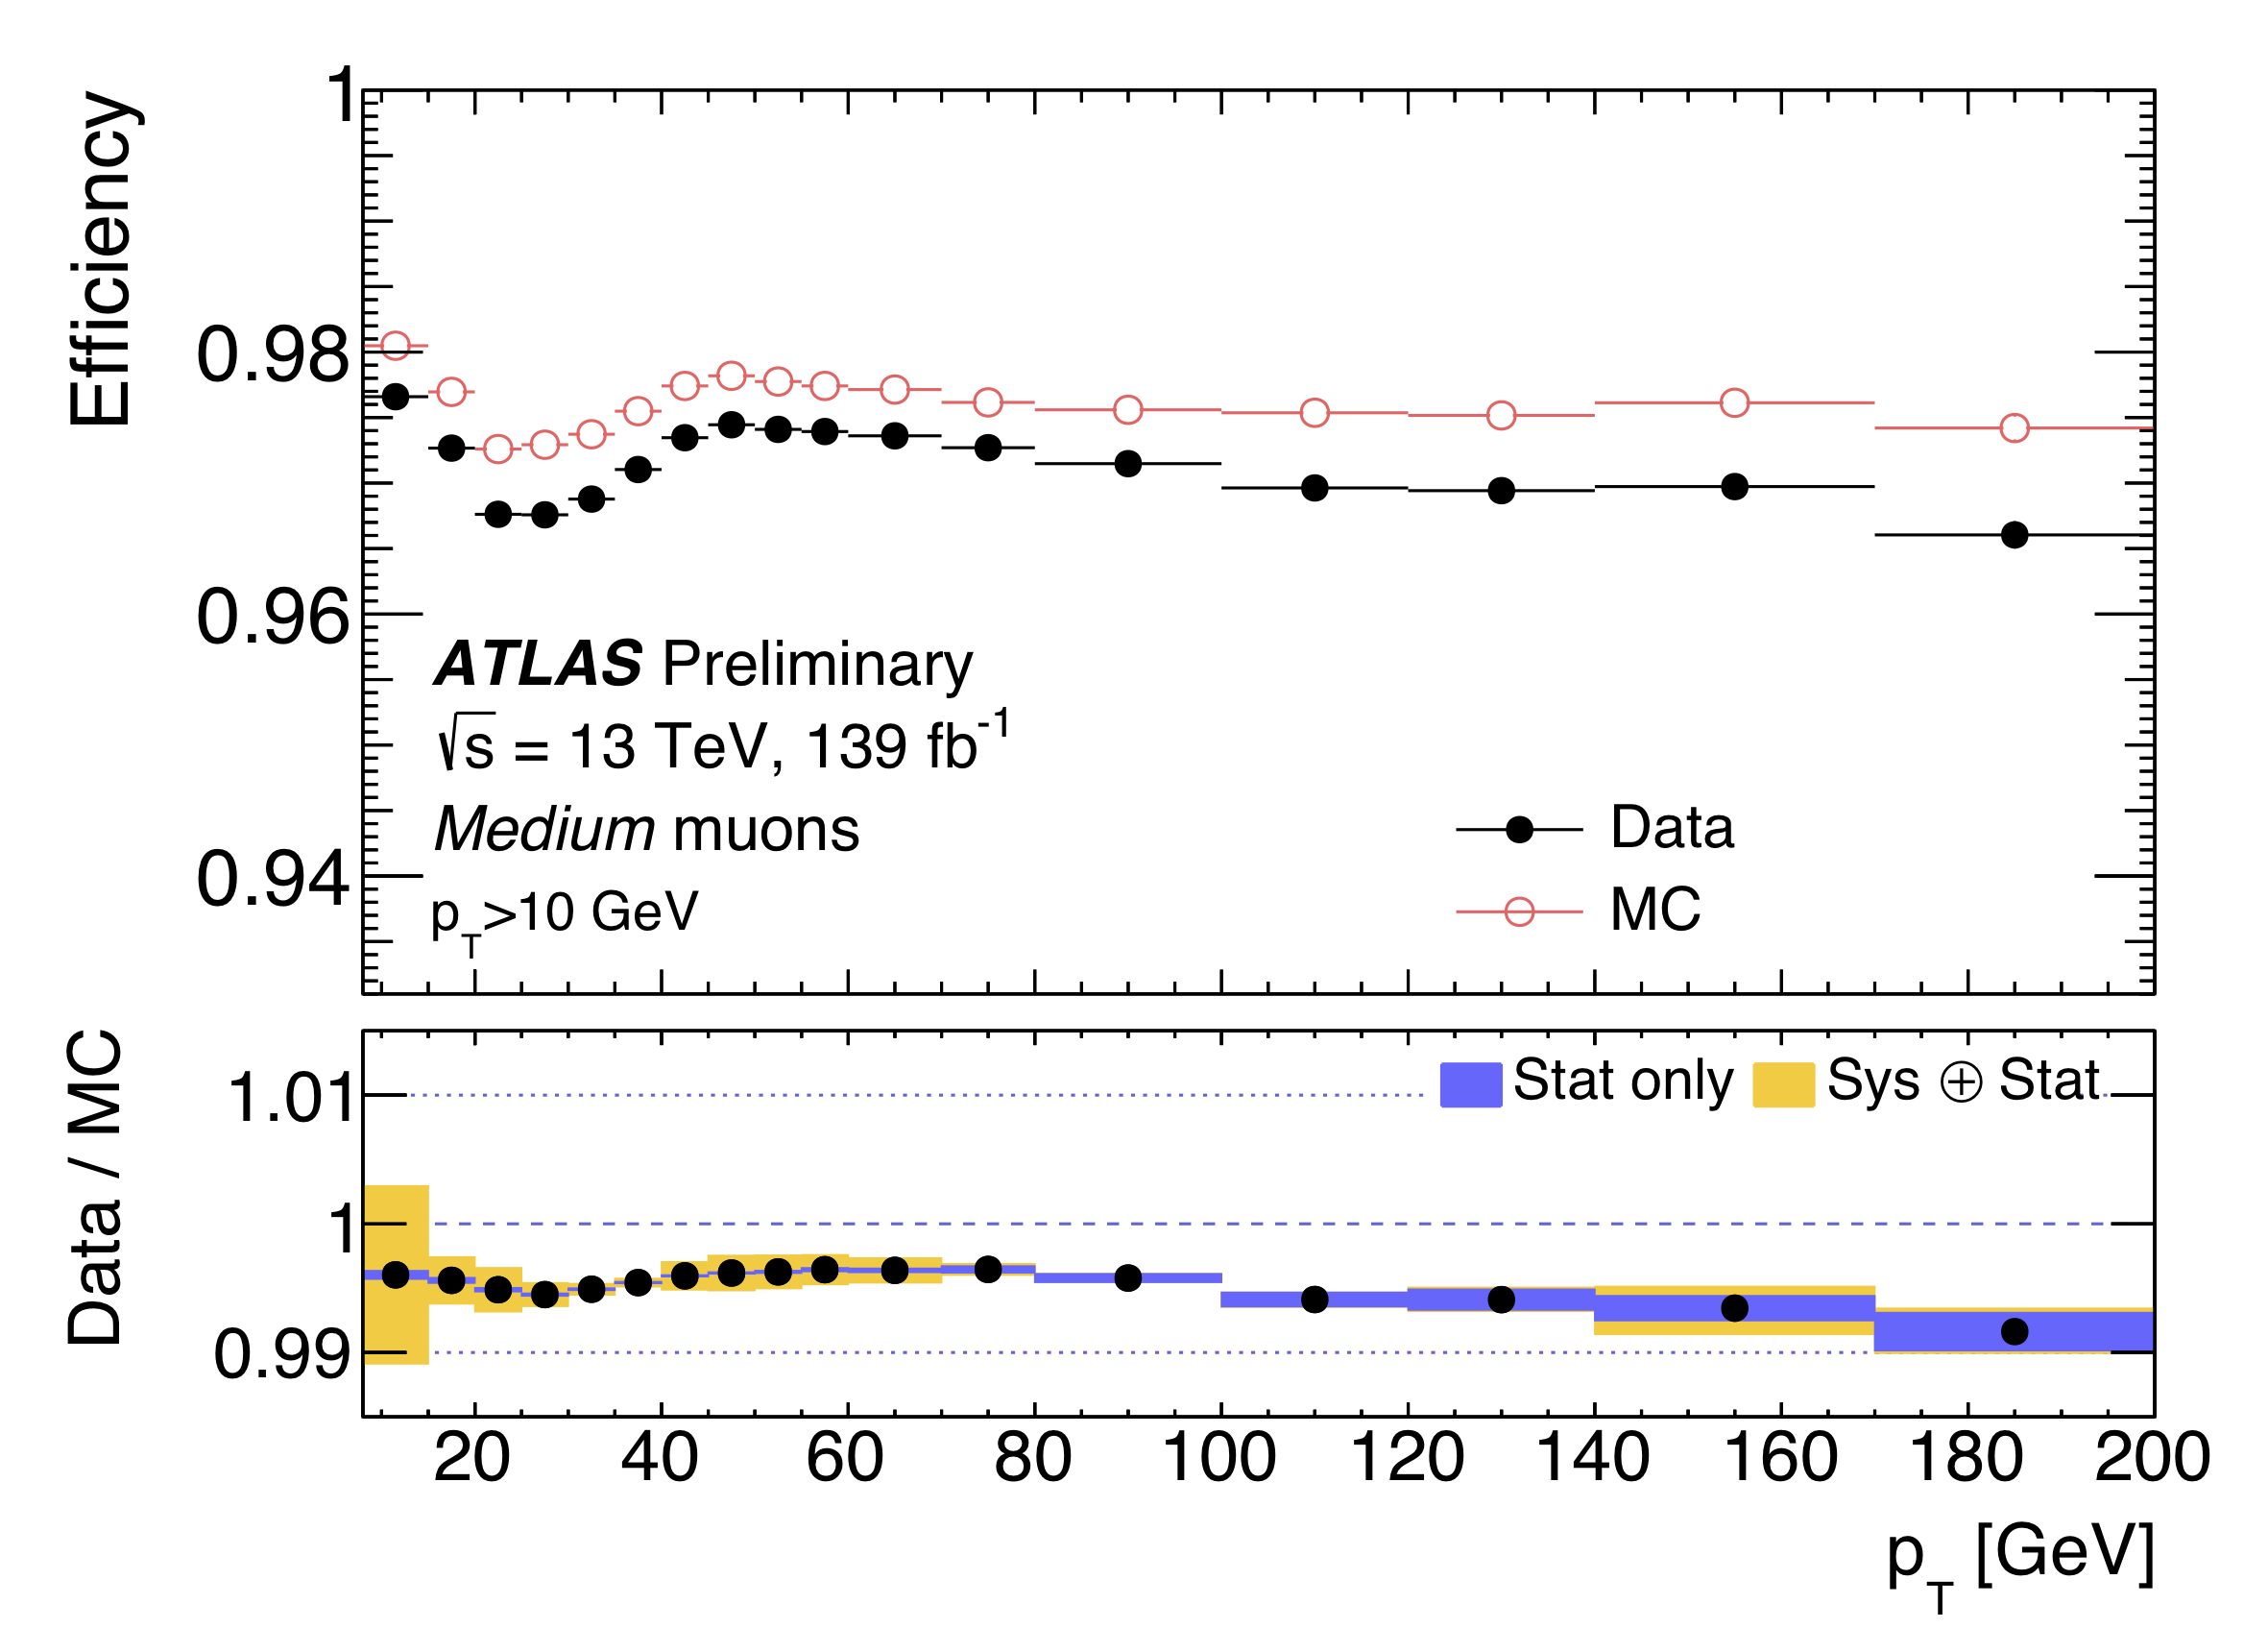
\includegraphics[width=\textwidth]{Pictures/efficiencyoverpt.PNG}
  \end{minipage}
  \hspace{.5cm}
  \begin{minipage}[b]{0.4\textwidth}
    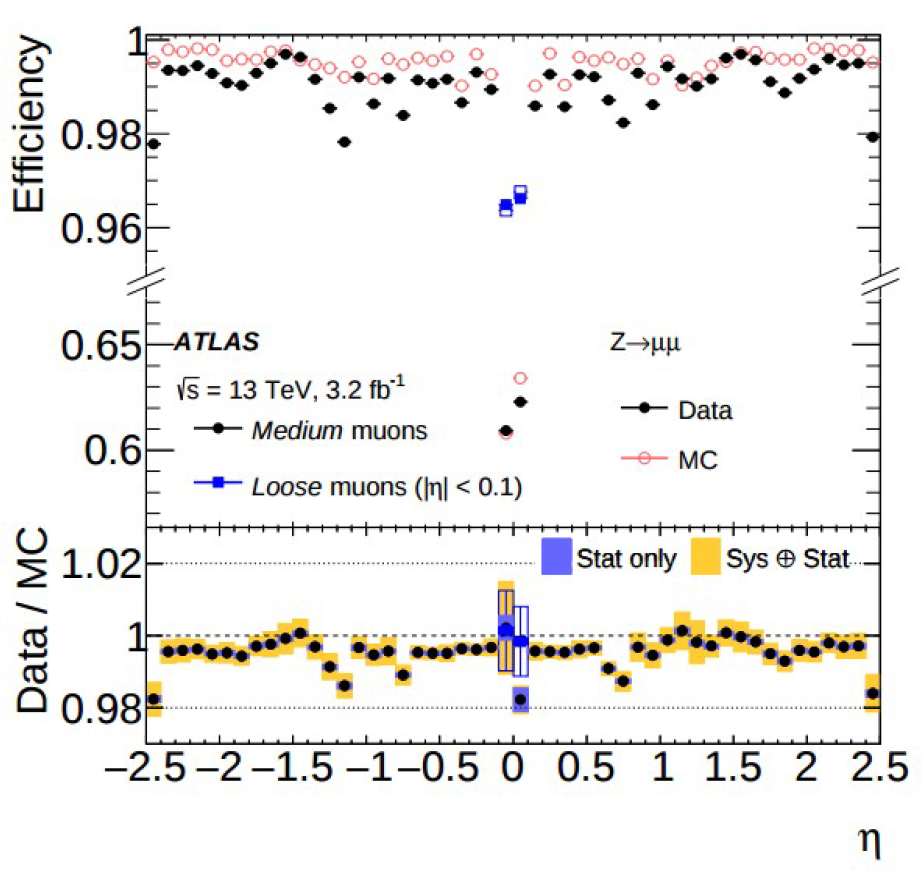
\includegraphics[width=\textwidth]{Pictures/efficiencyovereta.PNG}
  \end{minipage}
  \caption{On the left, reconstruction efficiency for \textit{Medium} muons from $Z \rightarrow \mu\mu$ and $J/\psi \rightarrow \mu\mu$ events is displayed as a function of the $p_T$ of the muon in the region $0.1 < |\eta| < 2.5$.  On the right, muon reconstruction efficiency is shown as a function of $\eta$ in $Z \rightarrow \mu\mu$ events for muons with $pT > 10$ GeV for \textit{Medium} and \textit{Loose} muons (squares) in the region $|\eta| < 0.1$, where the \textit{Loose} and \textit{Medium} selections differ significantly. In both plots the error bars on the efficiencies indicate the statistical uncertainty and the bottom panels show the ratio of the measured to predicted efficiencies, with both statistical and systematic uncertainties \cite{MCPpaper}.}
  \label{fig:efficiency}
\end{figure}

Figure \ref{fig:efficiency} displays reconstruction efficiency for \textit{Medium} muons over a range of $p_T$ and $\eta$. $J/\psi$ decays probe low $p_T$ muons while $Z$ decays probe muons of a higher $p_T$ allowing a large range to be defined.  Muon reconstruction works well over a large range of both $p_T$ and $\eta$ as evidenced by an efficiency above $95\%$ throughout ranges shown in $p_T$ and $\eta$. In addition, MC simulations match data quite well - within $1-2\%$. The only significant loss of efficiency is seen with \textit{Medium} muons at extremely low $\eta$ due to criteria excluding ID muons. We can make up this lost efficiency by substituting \textit{Loose} muons for excluded ID muons. Overall, the default \textit{Medium} muon selection demonstrates a high reconstruction efficiency. 

\subsubsection{Muon Isolation} \index{Isolation}
\par \hspace{20pt} Isolating muons from heavy particles is one of the keys to understanding the background in many physics analyses. When heavy particles like $W$, $Z$, and Higgs bosons decay they often produce muons in isolation. Semileptonic decays, on the other hand, typically produce muons embedded in jets.

\par \hspace{20pt} The MCP group uses two muon isolation variables: a track-based variable ($p_T^{varcone30}$) and a calorimeter-based variable ($E_T^{topocone20}$). $p_T^{varcone30}$ is defined as the scalar sum of the transverse momenta of tracks with $p_T > 1$ GeV in a cone around the muon of transverse momentum $p_T$ excluding the muon track itself. The cone size is $p_T$-dependent to improve the performance for muons produced in decays with a large transverse momentum. $E_T^{topocone20}$ is defined as the sum of the transverse energy of topological clusters in a cone around the muon after subtracting the contribution from the energy deposit of the muon itself and correcting for pile-up effects \cite{jets}. 

\par \hspace{20pt} Table \ref{tab:datasetsdef} defines seven isolation selection criteria - called ``isolation working points'' - that optimize different physics analyses. The\textit{LooseTrackOnly} and \textit{FixedCutTightTrackOnly} working points are defined by cuts on the relative track-based isolation variable. All other working points are defined by cuts applied separately on both relative isolation variables. All cuts are tuned as a function of the $\eta$ and $p_T$ of the muon to obtain a uniform performance. The target efficiencies of the different working points are described in Table \ref{tab:isolation}. The efficiencies for the seven isolation working points are measured in data and simulation using the \textbf{Tag-and-Probe} method described in Section \ref{sec:efficiency} on $Z \rightarrow \mu\mu$ decays. Figure \ref{fig:isolation} shows the isolation efficiency measured for \textit{Medium} muons in data and simulation as a function of the muon $p_T$ for two different working points. In both the \textit{Loose} and \textit{LooseTrackOnly} working points, efficiency is above $98\%$ and matches simulation well within errors. 

\begin{table}[!h]
	\centering 
    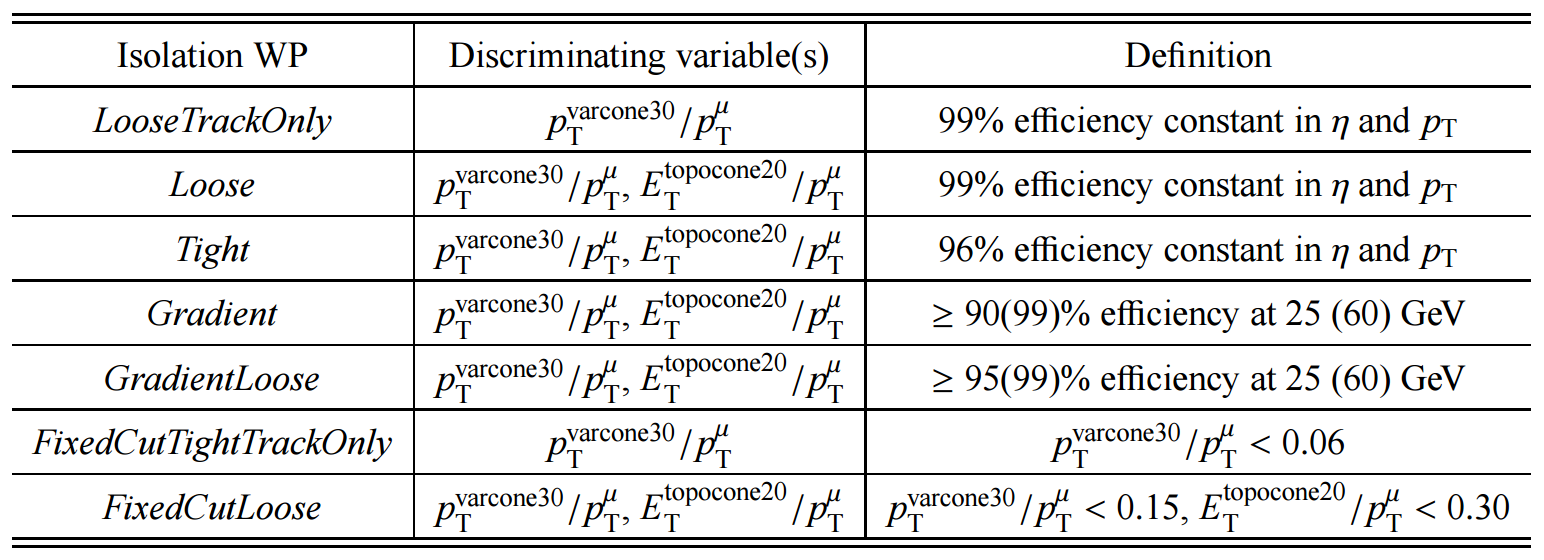
\includegraphics[width=.9\textwidth]{Pictures/isolationworkingpoints.PNG}
    \caption{The seven isolation working points are described by their discriminating variables and defining criteria \cite{MCPpaper}.}
    \label{tab:isolation}
\end{table}

\begin{figure}[!h]
  \centering
  \begin{minipage}[b]{0.47\textwidth}
    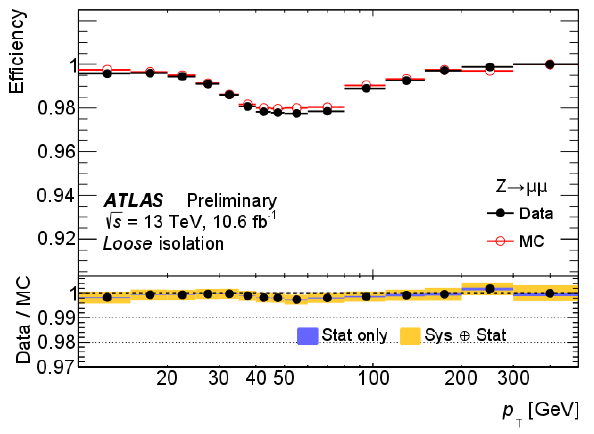
\includegraphics[width=\textwidth]{Pictures/isolationefficiency1.png}
  \end{minipage}
  \hspace{.2cm}
  \begin{minipage}[b]{0.48\textwidth}
    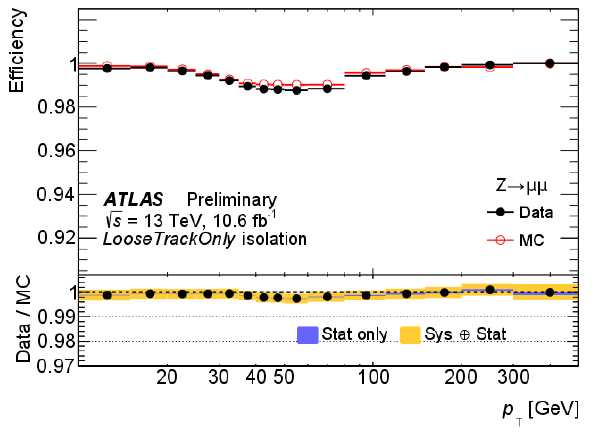
\includegraphics[width=\textwidth]{Pictures/isolationefficiency2.png}
  \end{minipage}
  \caption{Isolation efficiency for the Loose (left) and LooseTrackOnly (right) muon isolation working points. The efficiency is displayed as a function of $p_T$ in $Z \rightarrow \mu\mu$ events. The black markers show efficiency measured in data samples while the red show MC simulations. The bottom panel shows the ratio of the efficiency between the two as well as both  statistical and systematic uncertainties \cite{MCPpaper}.}
  \label{fig:isolation}
\end{figure}

\subsubsection{Muon Momentum Corrections} \index{Momentum Corrections}
\par \hspace{20pt} The muon momentum scale and resolution are studied using $Z$ and $J/\psi$ decays. In order to obtain agreement between simulation and data in muon momentum scale to the per mille level and in resolution to the percent level, we need to apply a set of corrections to the simulated muon momentum. After applying the corrections we validate them by comparing the muon momentum scale and resolution between simulation and data over $\eta$, $\phi$, and $p_T$.

\par \hspace{20pt} I have been heavily involved in calculating the parameters that govern the muon momentum corrections and validating them with the newest datasets. Within the next section, I will describe muon momentum corrections and the parametrizations that define them.

\par \hspace{20pt} We extract the calibration parameters with the transverse momentum of the ID and MS components of a CB track.  The corrected transverse momentum is described by the following equation: 

\begin{align*}
	\centering 
    p_T^{\textrm{Cor,Det}} = \frac{p_T^{\textrm{MC,Det}}+\sum\limits_{n=0}^1s_n^{\textrm{Det}}(\eta,\phi)(p_T^{\textrm{MC,Det}})^n}{1+\sum\limits_{m=0}^2\Delta r_m^{\textrm{Det}}(\eta,\phi)(p_T^{\textrm{MC,Det}})^{m-1}g_m} .
\end{align*}
\par \hspace{20pt} Here the $g_m$ terms are normally distributed random variables with zero mean and unit width. The $\Delta r $ and $s$ terms describe momentum resolution smearing and scale corrections applied in specific detector regions, respectively. Both the ID and MS are divided into $18$ pseudorapidity regions and the MS is divided into two $\phi$ bins separating the large and small sectors. Each of these bins leverages different alignment techniques and has different material distributions. 

\par \hspace{20pt} There are two $s$ terms that represent different types of corrections. $s_1$ corrects for inaccuracy in the description of the magnetic field integral and the detector in the direction perpendicular to the magnetic field. $s_0$ corrects for the inaccuracy in the simulation of energy loss in the calorimeter and other materials. Since this loss is negligible in the ID, it is only nonzero in the MS \cite{MCPpaper}.

\par \hspace{20pt} The denominator introduces momentum smearing which broadens the $p_T$ resolution in simulation. The parametrization of the smearing is defined:
\begin{align*}
	\centering 
    \frac{\sigma(p_T)}{p_T} = r_0/p_T \oplus r_1 \oplus r_2 \cdot p_T .
\end{align*}
In this equation $r_0$ is related to the fluctuations in energy loss in the traversed material, $r_1$ accounts for multiple scattering, local magnetic field inhomogeneities, and local radial displacements of hits, and $r_2$ describes intrinsic resolution effects caused by the spatial resolution of the hit measurements and by residual misalignment of the MS \cite{MCPpaper}. 

\par \hspace{20pt} Correction parameters are extracted from data using a binned maximum-likelihood fit with templates derived from simulation which compares the invariant mass distributions for $J/\psi$ and $Z$ decay candidates in data and simulation. The muons are carefully selected to be compatible with tracks that start at the interaction point and penetrate both the ID and the MS. Muons are also selected to pass specific momentum and isolation criteria. The dimuon mass distribution of these tracks in data is fitted using a Crystal Ball function convoluted with an exponential background distribution in the ID and MS fits. The background model and its normalization are then used in the template fit. The fits are performed in $\eta-\phi$ regions of fit (ROFs) which compromise regions with uniform features in the ID and MS \cite{MCPpaper}. 

\par \hspace{20pt} From these fits, we can find the smearing terms across all $\eta$ regions. Once the corrections are applied we can validate that the agreement between data and MC is excellent. This is shown in Figure \ref{fig:parametrizationeta}. $r_0$ is set to zero across all $\eta$ regions since energy loss is negligible in the ID. $r_1$ and $r_2$ increase as $\eta$ increases since spatial resolution decreases and inhomogeneities increase as as we move from the barrel to end-cap regions of both the ID and MS. 

\begin{figure}[!h]
	\centering 
    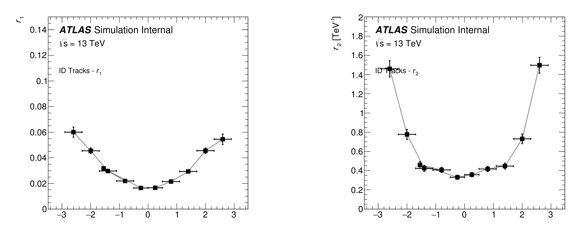
\includegraphics[width=.85\textwidth]{Pictures/parametrizationIDeta.PNG}
    \caption{ The $r$- values from each of $10$ fits of resolution to $p_T$ for ID muon simulations are shown. Each value corresponds to a particular ROF or $\eta$ region. These plots show $r_1$ (left) and $r_2$  (right) as functions of leading muon $\eta$.}
    \label{fig:parametrizationeta}
\end{figure}

\par \hspace{20 pt}
We must continue to study muon momentum corrections during ATLAS runs to validate muon calibration performance and account for discrepancies.
